\subsubsection{Navadne krivulje}
Novejši postopki so znatno olajšali izdelavo krivulj.
Lahko se izdelajo na CNC rezkalnem stroju na magnetni ali vakuumski mizi,
z žično erozijo, ki je nekoliko dražji a natančnejši postopek in tudi
obdelujemo lahko mnogo trše in trdnejše materiale ali pa tudi z
plamenskim in laserskim odrezom, kjer moramo po koncu izreza, površine
dodatno zbrusiti ročno, saj navadno te niso gladke.

Najbolj pogosto se izdelujejo iz jekla CK45 (1.1191), ki vsebuje
0.45 \% C, 0.65 \% Mn, 0.035 \% P in manj kot 0.035 \% S in ima natezno trdnost okoli 725 MPa.

Pred CNC stroji so krivulje izdelovali ročno na rezkalnih in vrtalnih strojih
in dokončno obdelali z ročnimi brusilkami.
Najprej se je ročno izrisala krivulja in se prenesla na surovec.
Če je bil surovec veliko večji od načrtovane krivulje, so se po
zunanji konturi izvrtale luknje tako, da so se približno 1-2mm
prekrivale. Potem se je krivulja, z kladivom in veliko tolčenja, izbila iz prvotnega surovca,
se vpela v primež in se z kotno brusilko izbrusila v končno obliko.

Spodaj, na sliki \ref{ploscate_krivulje} je prikazanih nekaj primerov
po meri izdelanih ploščatih krivulj.

\begin{figure}[H]
	\begin{center}
		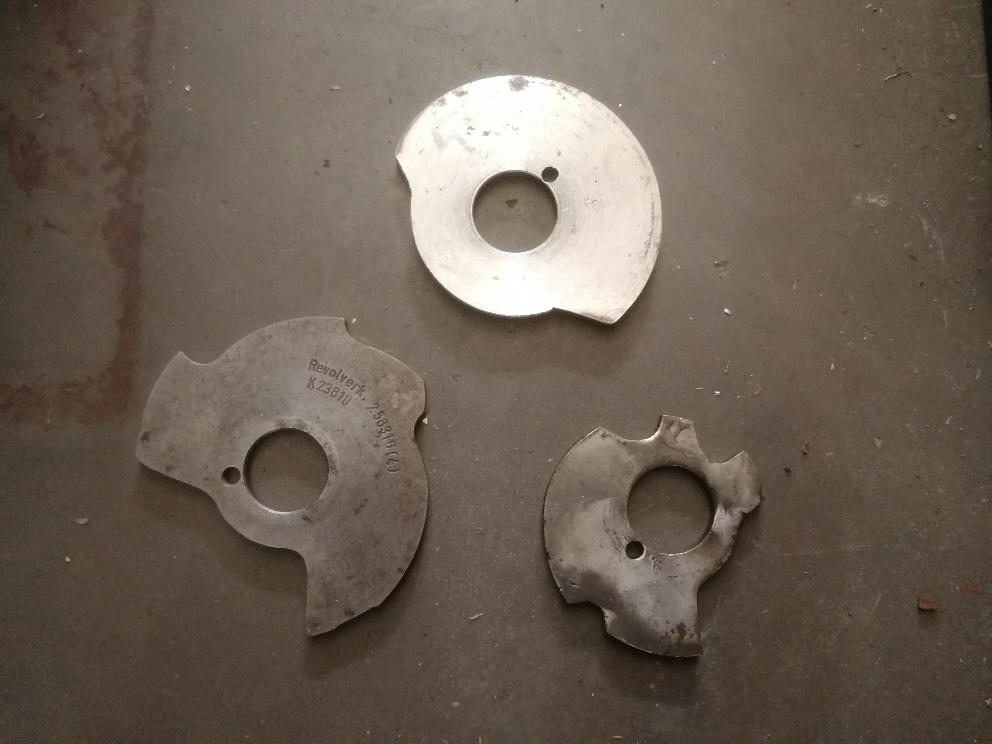
\includegraphics[width=13cm]{ploscate_krivulje.jpg}
		\caption{Ploščata krivulja
			\cite{lasten}}
		\label{ploscate_krivulje}
	\end{center}
\end{figure}

\subsubsection{Preračun navadnih krivulj}
\label{izracun_krivulj}
Primer: Imamo obdelovanec premera D - 12 mm, ki se vrti z hitrostjo S = 2000 \( \frac{obr}{min} \)
in časom enega cikla T - 30 s. Hočemo ga odrezati z odreznim nožem z pomikom f - 0.04 \( \frac{mm}{obr} \)
(Da stvar poenostavimo sem že izbral željen pomik na obrat, namesto da bi ga
izračunal iz rezalne hitrosti in premera)

Zaradi varnosti, bomo določili, da nož začne z delovnim gibom
na $\phi13$ in konča na $\phi-1$. To pomeni, da bo potoval 7 mm, ker
imamo simetrično obdelovanje.

Čas, potreben za ta gib izračunamo
\begin{equation}
	\label{cas_za_hod}
	\begin{split}
		t &= \frac{l*60s}{f*S} \\
		t &= \frac{7mm*60}{0.04\frac{mm}{obr}*2000\frac{obr}{min}} \\
		t &= 5.25s
	\end{split}
\end{equation}

Kolikšen kot krivulje mora obsegati vzpon, da bomo
dosegli željen pomik izračunamo
\begin{equation}
	\label{kot_krivulje}
	\begin{split}
		\alpha &= \frac{360\degree}{T} * t \\
		\alpha &= \frac{360\degree}{30s} * 5.25s \\
		\alpha &= 63\degree
	\end{split}
\end{equation}

Če imamo razmerje med vzvodi sledilca in nožem 1:1, potem se more krivulja v 63° vzpet za 7 mm.
Zdaj imamo dve možnosti:
\begin{itemize}
	\item Izdelamo krivuljo po meri.
	\item Izberemo najbližjo standardno krivuljo po raznih katalogih ali zalogi.
\end{itemize}

\subsubsection{Bobnaste krivulje}
Sodobna izdelava bobnastih krivulj poteka na CNC rezkalnih strojih
z vsaj štirimi osmi. Pred tem, pa so bobnaste krivulje večinoma delali v
odsekih in jih z tem ločili na hitre in delovne gibe in je bilo z tem
mogoče lažje in bolj natančno nastavljati zamike krivulj.
Možno je tudi, da se obrabljena krivulja enostavno zamenja brez
večjega zastoja. Po izdelavi se zakalijo na približno 50-60 HRC.

Na spodnji sliki \ref{bobnaste_krivulje} je prikazan primer
bobnaste krivulje.

\begin{figure}[H]
	\begin{center}
		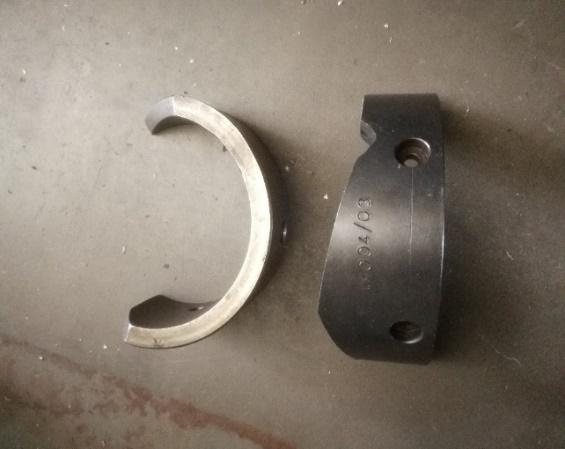
\includegraphics[width=10cm]{bobnasta_krivulja.jpg}
		\caption{Bobnasta krivulja
			\cite{lasten}}
		\label{bobnaste_krivulje}
	\end{center}
\end{figure}

\subsubsection{Kaljenje}
Po izdelavi se krivulje kalijo, da zmanjšamo obrabo in povečamo
obstojnost. Kaljenje je toplotna izdelava s katerim dosežemo utrjeno površino in
žilavo jedro. Obdelava je sestavljena z segrevanjem, zadrževanjem na temperaturi
kaljenja, hitrim ohlajanjem in popuščanjem, kot je vidno na spodnji
sliki \ref{diagram_kaljenja}. Po kaljenju dobimo fino zrnato strukturo jekla.

\begin{figure}[H]
	\begin{center}
		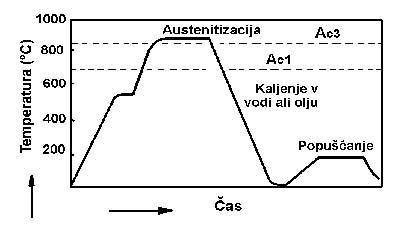
\includegraphics[width=10cm]{diagram_kaljenja.jpg}
		\caption{Diagram kaljenja z popuščanjem
			\cite{diagram_kaljenja}}
		\label{diagram_kaljenja}
	\end{center}
\end{figure}

Kalimo lahko na naslednje načine:
\begin{itemize}
	\item Kaljenje v pečeh.
	\item Induktivno Kaljenje.
	\item Plamensko kaljenje.
\end{itemize}

Na sliki \ref{induktivno_kaljenje} je prikazan primer induktivnega
segrevanja obdelovanca med bakrenimi obroči.

\begin{figure}[H]
	\begin{center}
		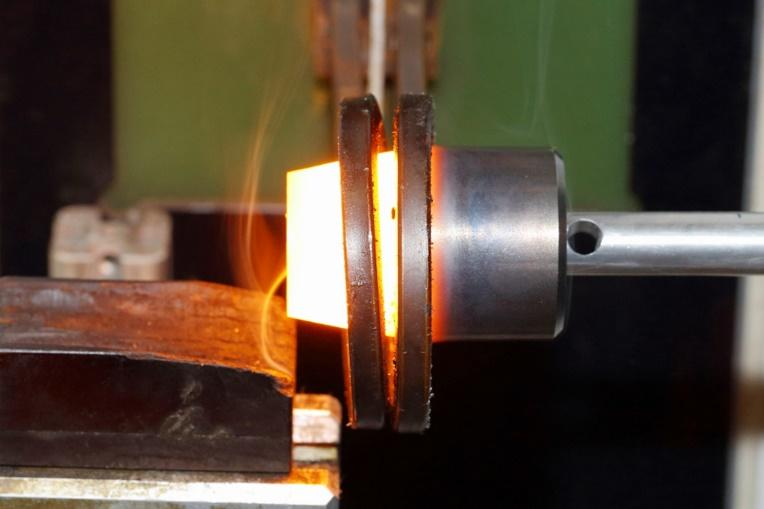
\includegraphics[width=10cm]{induktivno_kaljenje.jpg}
		\caption{Slika induktivnega kaljenja
			\cite{induktivno_kaljenje}}
		\label{induktivno_kaljenje}
	\end{center}
\end{figure}

Kaljenje v pečeh in induktivno kaljenje je v večji meri uporabno
za večje količine kosov. Omogoča namreč hitro in natančno kaljenje,
saj so sodobne peči elektronsko krmiljene in opremljene z raznimi senzorji.

Plamensko kaljenje se pa uporablja za manjše količine ali za
posamične kose, kateri ne potrebujejo natančne trdote. Za
segrevanje se uporablja plamenski gorilnik, z katerim segrejemo
material do določene barve in ga nato ohladimo v vodi ali v olju.

Temperature kaljenja so odvisne od jekla in njegovih legirnih
elementov. Segajo od 700 °C do 900 °C, temperature popuščanja
pa od 200 °C do 500 °C. Močnejše legirana jekla je potrebno
segrevati počasi do okolice 400 °C do 500 °C, da postane jeklo
duktilno nato ga lahko segrevamo hitreje.

Trajanje kaljenja je odvisno od debeline sten izdelka, njegove toplotne
prevodnosti in sredstva v katerem ga segrevamo. Pri prekratkem
segrevanju se notranjost predmetov ne segreje do zahtevane
temperature, kar privede do nepopolnega postopka obdelave. Pri
predolgem segrevanju pa se lahko pojavlja grobozrnata struktura
in delno razogličenje jekla.